\documentclass{article}
\usepackage{ae,aecompl}
\usepackage{todonotes}
\usepackage{chngcntr}
\usepackage{tikz-cd}
\usepackage{graphicx}
\graphicspath{ {./images/}}
\usepackage[all,cmtip]{xy}
\usepackage{amsmath, amscd}
\usepackage{amsthm}
\usepackage{amssymb}
\usepackage{amsfonts}
\usepackage{bm}
\usepackage{qsymbols}
\usepackage{latexsym}
\usepackage{mathrsfs}
\usepackage{mathtools}
\usepackage{cite}
\usepackage{color}
\usepackage{url}
\usepackage{enumerate}
\usepackage{verbatim}
\usepackage[draft=false, colorlinks=true]{hyperref}
\usepackage{pdfpages}
\usepackage[margin=1.2in]{geometry}
\usepackage{IEEEtrantools}

\usepackage{fancyhdr}


\usepackage[nameinlink]{cleveref}


\DeclareMathOperator*{\ac}{accept}
\DeclareMathOperator*{\amax}{argmax}
\DeclareMathOperator*{\amin}{argmin}
\DeclareMathOperator*{\Aut}{Aut}
\newcommand {\al}{{\alpha}}
\newcommand {\abs}[1]{{\left\lvert#1\right\rvert}}
\newcommand {\A}{{\mathcal{A}}}
\newcommand {\AM}{{\mathrm{AM}}}
\newcommand {\AMp}{{\AM_{p}^{X}\!(\Ri_\w)}}
\newcommand {\B}{{\mathcal{B}}}
\DeclareMathOperator*{\Be}{Bern}
\newcommand {\Br}{{\dot{B}}}
\newcommand {\Ba}{{\mathfrak{B}}}
\newcommand {\C}{{\mathbb C}}
\newcommand {\ce}{\mathrm{c}}
\newcommand {\Ce}{\mathrm{C}}
\newcommand {\Cc}{\mathrm{C_{c}}}
\newcommand {\Ccinf}{\mathrm{C_{c}^{\infty}}}
\DeclareMathOperator{\cov}{Cov}
\DeclareMathOperator{\DEV}{DEV}
\newcommand {\Di}{{\mathbb D}}
\newcommand {\dom}{\mathrm{dom}}
\newcommand{\dist}{\stackrel{\mathrm{dist}}{=}}
\newcommand {\ud}{\mathrm{d}}
\newcommand {\ue}{\mathrm{e}}
\newcommand {\eps}{\varepsilon}
\newcommand {\veps}{\varepsilon}
\newcommand {\vrho}{{\varrho}}
\newcommand {\E}{{\mathbb{E}}}
\newcommand {\Ec}{{\mathcal{E}}}
\newcommand {\Ell}{L}
\newcommand {\Ellp}{{L_{p}[0,1]}}
\newcommand {\Ellpprime}{{L_{p'}([0,1])}}
\newcommand {\Ellq}{{L_{q}([0,1])}}
\newcommand {\Ellqprime}{{L_{q'}([0,1])}}
\newcommand {\Ellr}{L^{r}}
\newcommand {\Ellone}{{L_{1}([0,1])}}
\newcommand{\Elltwo}{{L_{2}([0,1])}}
\newcommand{\Ellinfty}{L^{\infty}}
\newcommand{\Ellinftyc}{L_{\mathrm{c}}^{\infty}}
\newcommand{\exb}[1]{\exp\left\{#1\right\}}
\DeclareMathOperator*{\Ext}{Ext}
\newcommand{\F}{{\mathcal{F}}}
\newcommand{\Fe}{{\mathbb{F}}}
\newcommand{\G}{{\mathcal{G}}}
\newcommand{\HF}{\mathcal{H}_{\text{FIO}}^{1}(\Rd)}
\newcommand{\Hr}{H}
\newcommand{\HT}{\mathcal{H}}
\newcommand{\ui}{\mathrm{i}}
\newcommand{\I}{{I}}
\newcommand{\J}{{\mathcal{J}}}
\newcommand{\id}{{\mathrm{id}}}
\newcommand{\iid}{\stackrel{\mathclap{\normalfont\mbox{iid}}}{\sim}}
\newcommand{\im}{{\text{im }}}
\newcommand{\ind}{{\perp\!\!\!\perp}}
\DeclareMathOperator*{\Int}{int}
\newcommand{\intx}{{\overline{\int_{X}}}}
\newcommand{\inte}{{\overline{\int_{\E}}}}
\newcommand{\la}{\lambda}
\newcommand{\rb}{\rangle}
\newcommand{\lb}{{\langle}}
\newcommand{\La}{\Lambda}
\newcommand{\calL}{{\mathcal{L}}}
\newcommand{\lp}{{\mathcal{L}}^{p}}
\newcommand{\lpo}{{\overline{\mathcal{L}}^{p}\!}}
\newcommand{\Lpo}{{\overline{\Ell}^{p}\!}}
\newcommand{\M}{{\mathbf{M}}}
\newcommand{\Ma}{{\mathcal{M}}}
\newcommand{\N}{{{\mathbb N}}}
\newcommand{\Na}{{{\mathcal{N}}}}
\newcommand{\norm}[1]{\left\|#1\right\|}
\newcommand{\normm}[1]{{\left\vert\kern-0.25ex\left\vert\kern-0.25ex\left\vert #1 
    \right\vert\kern-0.25ex\right\vert\kern-0.25ex\right\vert}}
\newcommand{\Om}{{{\Omega}}}
\newcommand{\one}{{{\bf 1}}}
\newcommand{\pic}{\text{Pic }}
\newcommand{\ph}{{\varphi}}
\newcommand{\Pa}{{\mathbb{P}}}
\newcommand{\Po}{{\mathcal{P}}}
\newcommand{\Q}{{\mathbb{Q}}}
\newcommand{\R}{{\mathbb R}}
\newcommand{\Rd}{{\mathbb{R}^{d}}}
\DeclareMathOperator{\rej}{reject }
\newcommand{\Rn}{{\mathbb{R}^{n}}}
\newcommand{\cR}{{\mathcal{R}}}
\newcommand{\Rad}{{\mathrm{Rad}}}
\newcommand{\ran}{{\mathrm{ran}}}
\newcommand{\Ri}{{\mathrm{R}}}
\newcommand{\supp}{{\mathrm{supp}}}
\newcommand{\Se}{\mathrm{S}}
\newcommand{\Sp}{S^{*}(\Rn)}
\newcommand{\St}{{\mathrm{St}}}
\newcommand{\Sw}{\mathcal{S}}
\newcommand{\T}{{\mathcal{T}}}
\newcommand{\ta}{{\theta}}
\newcommand{\Ta}{{\Theta}}
\newcommand{\topp}{\stackrel{p}{\to}}
\newcommand{\todd}{\stackrel{d}{\to}}
\newcommand{\toL}[1]{\stackrel{L^{#1}}{\to}} 
\newcommand{\toas}{\stackrel{a.s.}{\to}}
\DeclareMathOperator{\V}{Var}
\newcommand {\w}{{\omega}}
\newcommand {\W}{{\mathrm{W}}}
\newcommand {\Wnp}{\text{$\mathrm{W}$\textsuperscript{$n,\!p$}}}
\newcommand {\Wnpeq}{\text{$\mathrm{W}$\textsuperscript{$n\!,\!p$}}}
\newcommand {\Wonep}{\text{$\mathrm{W}$\textsuperscript{$1,\!p$}}}
\newcommand {\Wonepeq}{\text{$\mathrm{W}$\textsuperscript{$1\!,\!p$}}}
\newcommand {\X}{{\mathcal{X}}}
\newcommand {\Z}{{{\mathbb Z}}}
\newcommand {\Za}{{\mathcal{Z}}}
\newcommand {\Zd}{{\Z[\sqrt{d}]}}
\newcommand {\vanish}[1]{\relax}

\newcommand {\wh}{\widehat}
\newcommand {\wt}{\widetilde}
\newcommand {\red}{\color{red}}

% Distributions
\newcommand{\normal}{\mathsf{N}}
\newcommand{\poi}{\mathsf{Poisson}}
\newcommand{\bern}{\mathsf{Bernoulli}}
\newcommand{\bin}{\mathsf{Binomal}}
\newcommand{\multi}{\mathsf{Multinomial}}
\newcommand{\Exp}{\mathsf{Exp}}



% put your command and environment definitions here




% some theorem environments
% remove "[theorem]" if you do not want them to use the same number sequence


  \newtheorem{thrm}{Theorem}
  \newtheorem{lemma}{Lemma}
  \newtheorem{prop}{Proposition}
  \newtheorem{cor}{Corollary}

  \newtheorem{conj}{Conjecture}
  \renewcommand{\theconj}{\Alph{conj}}  % numbered A, B, C etc

  \theoremstyle{definition}
  \newtheorem{defn}{Definition}
  \newtheorem{ex}{Example}
  \newtheorem{exs}{Examples}
  \newtheorem{question}{Question}
  \newtheorem{remark}{Remark}
  \newtheorem{notn}{Notation}
  \newtheorem{exer}{Exercise}




\title{STATS305A - Lecture 8}
\author{John Duchi\\ Scribed by Michael Howes}
\date{10/14/21}

\pagestyle{fancy}
\fancyhf{}
\rhead{STATS305A - Lecture 8}
\lhead{10/14/21}
\rfoot{Page \thepage}

\begin{document}
\maketitle
These were updated on 10/15/21 to reflect the new notes on Scheffe's method that John uploaded after class.
\tableofcontents
\section{Announcements}
Etude due tonight. 
John's null hypothesis for today $H_0:$ It is intelligent to wear headphones while biking! John is confident that this null hypothesis can be rejected.
\section{Multiple Hypothesis Testing}
\subsection{Motivation}
In the linear model $Y=X\beta + \eps$ we are often interested in many parameters. For example if the coordinate $j$ associated with the response $Y$ for $j=1,\ldots,d$.

Another way to say this is that we wish to test many nulls. For example
\begin{align*}
    H_{0,1} &: \beta_1 = 0, \beta_0, \beta_2,\ldots, \beta_d \text{ arbitrary}.\\
    H_{0,2} &: \ldots\\
    \vdots &  \\
    H_{0,j} &: \beta_j = 0, \beta_{\setminus j} \text{ arbitrary}\\
    \vdots & \\
    H_{0,d}&:\ldots
\end{align*}
The notation $\beta_{\setminus j}$ means all $\beta_i$ apart from $\beta_j$. 

\underline{Issue/problem} If we perform $d$ distinct hypothesis tests, each of which we reject at level $\al$, then we expect as many as $d\al$ false rejections.

\subsection{Why most published research is false}
See: Ioanndis 2005 on course webpage. Setting: $H_{0,1},H_{0,2},\ldots,H_{0,d}$ null hypotheses. Rejecting a null means making a discovery. We would like to understand 
\[\Pa(H \text{ is false}| H \text{ is rejected}). \]
Saw we use $\al$-level test with $\beta$ power. That is 
\begin{align*}
    \beta &= \Pa(\text{reject }| H \text{ is false}).\\
    \al &= \Pa(\text{reject }| H \text{ is true}).
\end{align*} 
Suppose also there is some value $\phi = $ frequency of \emph{actually} false hypothesis = frequency of true scientific discoveries. By Bayes rule
\begin{align*}
    \Pa(H \text{ is false }| H \text{ rejected}) & = \frac{\Pa(H \text{ rejected }|H \text{ is false})\Pa(H \text{ is false})}{\Pa(H \text{ rejected})}\\
    &=\frac{\Pa(H \text{ rejected }|H \text{ is false})\Pa(H \text{ is false})}{\Pa(H \text{ rejected }|H \text{ is false})\Pa(H \text{ is false})+\Pa(H \text{ rejected }|H \text{ is true})\Pa(H \text{ is true})}\\
    &=\frac{\beta \phi}{\beta \phi + \al(1-\phi)}
\end{align*}
Define $p_\beta(\phi) = \frac{\beta \phi}{\beta \phi + \al(1-\phi)}$. We wish to understand this curve as a function of $\phi$. Suppose that $\beta=1$ and so if the null is false we will always correctly reject (if there is a true discovery to be discovered, we will discover it.) Then 
\[p(\phi) = \frac{\phi}{\phi+\al(1-\phi)}. \]
If $\al = 0.05$, the plot of this function looks like this:
\begin{center}
   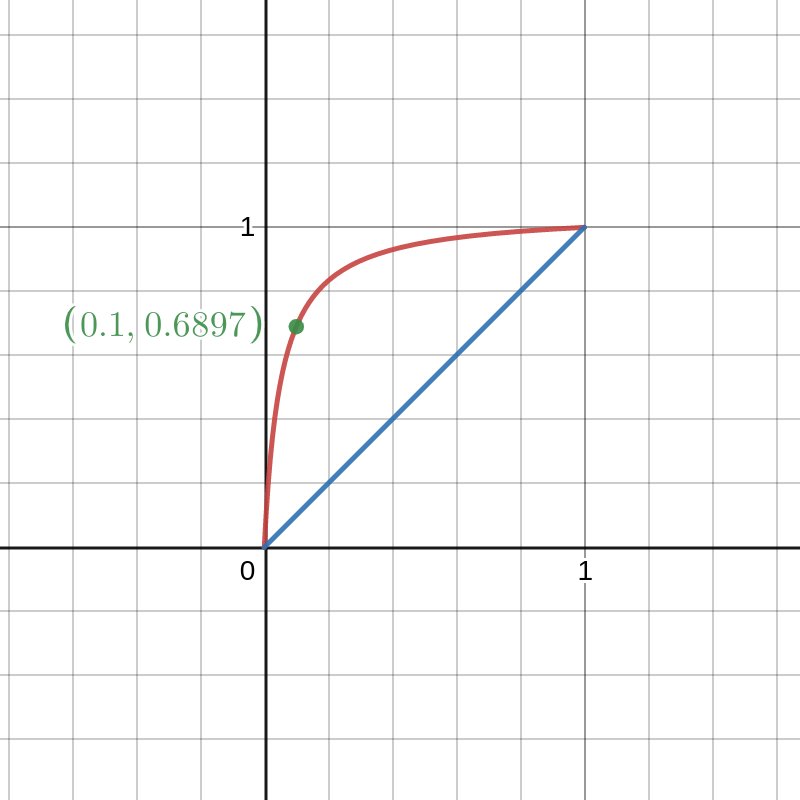
\includegraphics[width = \textwidth/2]{10_14_P01.png}
\end{center}
If $\phi = 0.1$ so 1/10 of the hypotheses we generate correspond to true discoveries. Then \[p(0.1) = \frac{0.1}{0.1+0.05\times 0.9} \approx \frac{2}{3}.\]
Thus given that we reject a hypothesis, there is a $\frac{2}{3}$ chance that we have made a true discovery (ie a $\frac{1}{3}$ chance we haven't discovered anything).

\begin{ex}
    Consider a genetics experiment such as a GWAS. We may have $d=10000$ genes and we wish to find the genes that are implicated in a disease. There may only be one such gene.  Thus $\phi = 1/10000$. Thus 
    \begin{align*}
        \Pa(\text{false discovery})&= \Pa(H \text{ is false }| H \text{ rejected})\\
        &= 1-\frac{1}{1+\al\frac{1-\phi}{\phi}}\\
        &\approx 1-\frac{1}{1+\al\cdot 10000}\\
        &\approx 1 \quad \text{unless $\al$ is very small}.
    \end{align*}
    Even if we do make $\al$ very very small, there are problem since multiple people are doing multiple studies and so  again the false discovery rate goes up. 

    Some comments from students: In actual GWAS studies, the first experiement is done to find a gene that might be implicated in a disease. In a second independent experiment that one gene is tested for significance. This brings the number of hypotheses down from 10000 to 1 and helps control false discoveries.

    Another comment: Sometimes the genes are grouped into clusters and we then examine which clusters are associated with the disease. This again reduces the number of tests. We will see this idea of grouping inputs later in class.

    We will still have the problem of multiple people performing multiple experiments which increases the false discovery rate.
\end{ex}
\section{Corrections}
How can we deal with these problems?

\subsection{Bonferroni correction (union bound)}
Say we have nulls $H_{0,j}, j = 1,\ldots,k$. Then 
\begin{align*}
    \Pa(\text{any } H_{0,j} \text{ falsely rejected})& \le \sum_{j=1}^k \Pa(H_{0,j} \text{ falsely rejected})\\
    &\le \sum_{j=1}^k a_j \quad \text{ if test $j$ is level $\al_j$}.
\end{align*}
Thus one solution is to choose level $\al_j$ tests so that $\sum_{j=1}^k \al_j = \al$. Usually when people do Bonferroni corrections they take $\al_j = \al/k$ for all $j$. This correction controls the FWER (family wise error rate). With this correction we know 
\[\Pa(\text{\emph{any} false discovery}) \le \al. \]
\subsection{Scheffe's method}
If we go back to the linear model we can make more specialised tests/corrections.

Suppose we want to simultaneously test a bunch of constrasts (ie linear functions). For $\Lambda \in \R^{d \times k}$ we want to test 
\[\lambda^T\beta = 0,\]
for all $\lambda \in \spn(\Lambda)$. This is \emph{a lot} of hypotheses. 

Suppose that $\text{rank}(\Lambda) = r$ and that $\spn(\Lambda) \subseteq \spn(X^T)$ and so $\Lambda$ is estimable. We have our usual $t$-test to test $\lambda^T\beta = 0$. Note that 
\[\lambda^T \beta = 0 \text{ for all } \la \in \spn(\Lambda) \Longleftrightarrow \Lambda^T\beta  = 0. \]
We can test $\Lambda^T \beta = 0$ by the $F$-test. Find $C \in \R^{n \times k}$ so that $\Lambda = X^TC$ and define $\wh{\theta} = C^TY$. We know $\E[\wh{\theta}] = C^TX\beta = \Lambda^T\beta$. The $F$-test tells us we need to look at the ratio between $\norm{\wh{\ta}}_2^2$ and $\norm{Y-\wh{Y}}_2^2$.\\

\underline{How do we actually implement this?}
We will first look at the distribution of $\Lambda^T \wh{\beta}$ under the null $H_0 :\Lambda^T \beta = 0$.  We will use the fact that $(X^TX)^\dagger = X^\dagger (X^\dagger)^T$. This is true because if $X = U\Sigma V^T$, then 
\[X^\dagger (X^\dagger)^T = V\Sigma^\dagger U^T U \Sigma^\dagger V^T = V(\Sigma^2)^\dagger V^T = (V\Sigma^2 V^T)^\dagger = (X^TX)^\dagger. \]
We claim that $\Lambda^T \wh{\beta} \sim \Na(0, \sigma^T \Lambda^T(X^TX)^\dagger \Lambda)$. Note that  $\beta = X^\dagger Y$ and that $X^TX(X^TX)^\dagger \Lambda= \Lambda$ since $\Lambda$ is in the range of $X^T$. and $(X^TX)(X^TX)^\dagger$ is the projection onto $\range(X^T)$. It follows that 
\[\Lambda^T\wh{\beta} = \Lambda^T X^\dagger Y = \Lambda^T X^\dagger X \beta + \Lambda^T X^\dagger \eps = \Lambda^T\beta + \Lambda^T X^\dagger \eps = \Lambda^T X^\dagger \eps, \]
under $H_0$. It follows that $\Lambda^T \wh{\beta}$ is normal with mean 0 and variance $\sigma^r \Lambda^T X^\dagger (X^\dagger)^T \Lambda = \sigma^2 \Lambda^T (X^TX)^\dagger \Lambda$. 

Furthermore if we define $H=XX^\dagger = $ projection onto $\spn(X)$, then \[(I-H)Y = (I-H)\eps \sim N(0,\sigma^2(I-H))\] and
\[\text{Cov}((I-H)Y,\Lambda^T\wh{\beta}) = \E[(I-H)\eps\eps^T(X^\dagger)^T\Lambda] =\sigma^2(I-H)(X^\dagger)^T\Lambda = 0. \]
Thus $(I-H)Y$ and $\Lambda^T \wh{\beta}$ are independent under the null $H_0 : \Lambda^T\beta = 0$. Thus we have the following:
\begin{prop}
    Under the null $H_0 : \Lambda^T \beta = 0$, the statistic 
    \begin{equation}\label{F-stat}
        T := \frac{\frac{1}{r}(\Lambda^T\wh{\beta})^T(\Lambda^T (X^TX)^\dagger \Lambda)^\dagger \Lambda^T \wh{\beta}}{\frac{1}{n-r(X)}\norm{(I-H)Y}_2^2},
    \end{equation}
    has an $F_{r,n-r(X)}$ distribution where $r$ is the rank of $\Lambda$ and $r(X)$ is the rank of $X$.
\end{prop}
Note that this result holds even if $X$ and $\Lambda$ are low rank. The only requirement is that $\Lambda$ is estimable. That is $\spn(\Lambda) \subseteq \spn(X^T)$. 

\begin{ex}
    Suppose we are doing ANOVA with $k$ groups. And so 
    \[X=\begin{bmatrix}
        1&1&0&\ldots& 0\\
        1&1&0&\ldots&0\\
        \vdots&\vdots &\vdots&\vdots&0\\
        1&1&0&\ldots&0\\
        1&0&1&\ldots&0\\
        1&0&1&\ldots&0\\
    
        \vdots&\vdots &\vdots&\ddots&0\\
        1&0&0&\ldots&1\\
        1&0&0&\ldots&1
    \end{bmatrix} \]
    $Y_{i,j} = \mu+\al_i + \eps_{i,j}$, $i=1,\ldots,k$, $j=1,\ldots, n_i$ and $X \in \{0,1\}^{N \times k + 1}$ where $N = \sum_{i=1}^k n_i$. Define 
    \[\Lambda = [e_2-e_3, e_2-e_4,\ldots, 3_2-e_{k+1}, e_3-e_4,\ldots, \ldots, e_k - e_{k+1}] \in R^{(k+1) \times \frac{k(k-1)}{2}}. \]
    That is $\Lambda$ is a matrix of differences that tests the hypotheses $\al_i -  \al_{i'} = 0$. Note $\text{rank}(\Lambda) << \frac{k(k-1)}{2}$ and $\text{rank}(X) = k < k+1$, so both are low rank. We also have
    \[
    X^TX = \begin{bmatrix*}
        N  &n_1&n_2&\ldots& n_k\\
        n_1&n_1&0&\ldots &0\\
        n_1&0  &n_2&\ldots &0\\
        \vdots &\vdots&\vdots &\ddots &\vdots\\
        n_k&0&0&\ldots &n_k
    \end{bmatrix*}\in \R^{(k+1)\times(k+1)},
    \]
    and
    \[\Lambda^T\wh{\beta} = \begin{bmatrix}
        \wh{\al}_1-\wh{\al}_2\\
        \wh{\al}_1-\wh{\al}_3\\
        \vdots \\
        \wh{\al}_{k-1}-\wh{\al}_k
    \end{bmatrix}\in \R^{k(k-1)/2}, \]
    and
    \begin{align*}
        \Lambda^T (X^TX)^\dagger \Lambda &= \Lambda^T\begin{bmatrix}
            0&0&\ldots &0\\
            0&n_1&\ldots &0\\
            \vdots &\vdots & \ddots & \vdots \\
            0&0&\ldots& n_k
        \end{bmatrix}^\dagger \Lambda\\
        &=\Lambda^T\begin{bmatrix}
            0&0&\ldots &0\\
            0&1/n_1&\ldots &0\\
            \vdots &\vdots & \ddots & \vdots \\
            0&0&\ldots& 1/n_k
        \end{bmatrix} \Lambda
    \end{align*}
\end{ex}
We are now ready to state \underline{Scheffe's method}:\\

Declare $\la \in \spn(\Lambda)$ significant if 
\begin{equation}\label{scheffe}
    \frac{
        \frac{(\la^T \wh{\beta})^2}{r\la^T(X^TX)^{\dagger}\la}
    }{\frac{1}{r-\text{rank}(X)}\norm{(I-H)Y}_2^2} > F \text{ threshold with $\al$ level, $r, n-\text{rank}(X)$ degrees of freedom.} 
\end{equation}
Scheffe's test rejects at level $\al$ iff the F test in equation \eqref{F-stat} rejects at the level $\al$.
\begin{proof}
    Consider maximizing 
    \[\frac{(\la^T \wh{\beta})^2}{\la^T X(^TX)^\dagger \la} \]
    over $\la \in \spn(\Lambda)$. We have assumed $\spn(\Lambda) \subseteq \spn(X^T)$. Let $X=U\Sigma V^T$ and take $\la = \Lambda w$ for some vector $w$. Define
    \[v:= (\Lambda^T(X^TX)^\dagger \Lambda)^{1/2}w, \]
    and so
    \[w= ((\Lambda^T(X^TX)^\dagger\Lambda)^{1/2})^\dagger v = (\Lambda^T(X^TX)^\dagger\Lambda)^{\dagger/2} v. \]
    Thus
    \[\frac{(w^T\Lambda^T \wh{\beta})^2}{w^T\Lambda^T (X^TX)^\dagger \Lambda w} = \frac{(v^T(\Lambda^T(X^TX)^\dagger\Lambda)^{\dagger/2}\Lambda^T\wh{\beta})^2}{\norm{v}^2_2}. \]
    By Cauchy-Schwarz, we have 
    \begin{align*}
        ((v^T(\Lambda^T(X^TX)^\dagger\Lambda)^{\dagger/2})\Lambda^T\wh{\beta})^2 
        \le& \norm{v}_2^2 \norm{(\Lambda^T(X^TX)^\dagger\Lambda)^{\dagger/2})\Lambda^T\wh{\beta}}_2^2\\
         =&\norm{v}_2^2 ((\Lambda^T(X^TX)^\dagger\Lambda)^{\dagger/2}\Lambda^T\wh{\beta})^T(\Lambda^T(X^TX)^\dagger\Lambda)^{\dagger/2}\Lambda^T\wh{\beta}\\
         =&\norm{v}_2^2(\Lambda^T\wh{\beta})^T(\Lambda^T(X^TX)^\dagger\Lambda)^{\dagger}\Lambda^T\wh{\beta}.
    \end{align*}
    Thus combining all we have done we have
    \[\frac{(\la^T \wh{\beta})^2}{\la^T X(^TX)^\dagger \la} \le \frac{\norm{v}_2^2}{\norm{v}_2^2}(\Lambda^T\wh{\beta})^T(\Lambda^T(X^TX)^\dagger\Lambda)^{\dagger}\Lambda^T\beta=(\Lambda^T\wh{\beta})^T(\Lambda^T(X^TX)^\dagger\Lambda)^{\dagger}\Lambda^T\beta. \]
    And we can conclude that the ratio in \eqref{scheffe} is always less than or equal to the ratio in \eqref{F-stat}. Furthermore we have equality when 
    \[v=(\Lambda^T(X^TX)^\dagger\Lambda)^{\dagger/2} \Lambda^T\wh{\beta}, \]
    and so we are done.
\end{proof}
Note: Often Scheffe's test is too conservative and it fails to reject some interesting stuff.
\begin{ex}
    Continuing our ANOVA example. In our example $\spn(\Lambda)$ is equal to $\la = [\la_0,\la_1,\ldots, \la_k]^T$ such that $\la_0=0$ and $\one^T \la =0$. Thus
    \[\la^T\wh{\beta} = \sum_{i=1}^k \la_i \wh{\al}_i = \sum_{i=1}^k \la_i \bar{Y}_i. \]
    Also recall that 
    \[
        X^TX = \begin{bmatrix*}
            N  &n_1&n_2&\ldots& n_k\\
            n_1&n_1&0&\ldots &0\\
            n_1&0  &n_2&\ldots &0\\
            \vdots &\vdots&\vdots &\ddots &\vdots\\
            n_k&0&0&\ldots &n_k
        \end{bmatrix*}\in \R^{(k+1)\times(k+1)},
        \]
        and 
        \[
           \la^T(X^TX)^\dagger \la = \la^T\begin{bmatrix}
                0&0&\ldots &0\\
                0&1/n_1&\ldots &0\\
                \vdots &\vdots & \ddots & \vdots \\
                0&0&\ldots& 1/n_k
            \end{bmatrix} \lambda = \sum_{i=1}^k \frac{\la_i^2}{n_i}.
            \]
        Thus our statistic from Scheffe's method is
        \[\frac{
            \frac{(\la^T \wh{\beta})^2}{r\la^T(X^TX)^{-1}\la}
        }{\frac{1}{r-\text{rank}(X)}\norm{(I-H)Y}_2^2}=\frac{
            \frac{(\sum_{i=1}^k \la_i\bar{Y}_i)^2}{r\sum_{i=1}^k \frac{\la_i^2}{n_i}}
        }{\frac{1}{r-k}\norm{(I-H)Y}_2^2}. \]
        Exercise find the $\la$ that maximizes the ratio: 
        \[ \frac{(\sum_{i=1}^k \la_i\bar{Y}_i)^2}{r\sum_{i=1}^k \frac{\la_i^2}{n_i}},\]
        subject to $\la^T \one = 0$.
\end{ex}
 \end{document}